\chapter{SYSTEM DESIGN}\label{ch:design}
\begingroup\emergencystretch=3em

\section{System Architecture}\label{sec:architecture}
The system architecture connects live video capture, preprocessing, AI detection, post-processing,
overlay visualization, and the user interface. Figure~\ref{fig:architecture} presents the
architecture overview. The layered diagram describes how
visual input is transformed into information displayed to the user.

\begin{figure}[htbp]
  \centering
  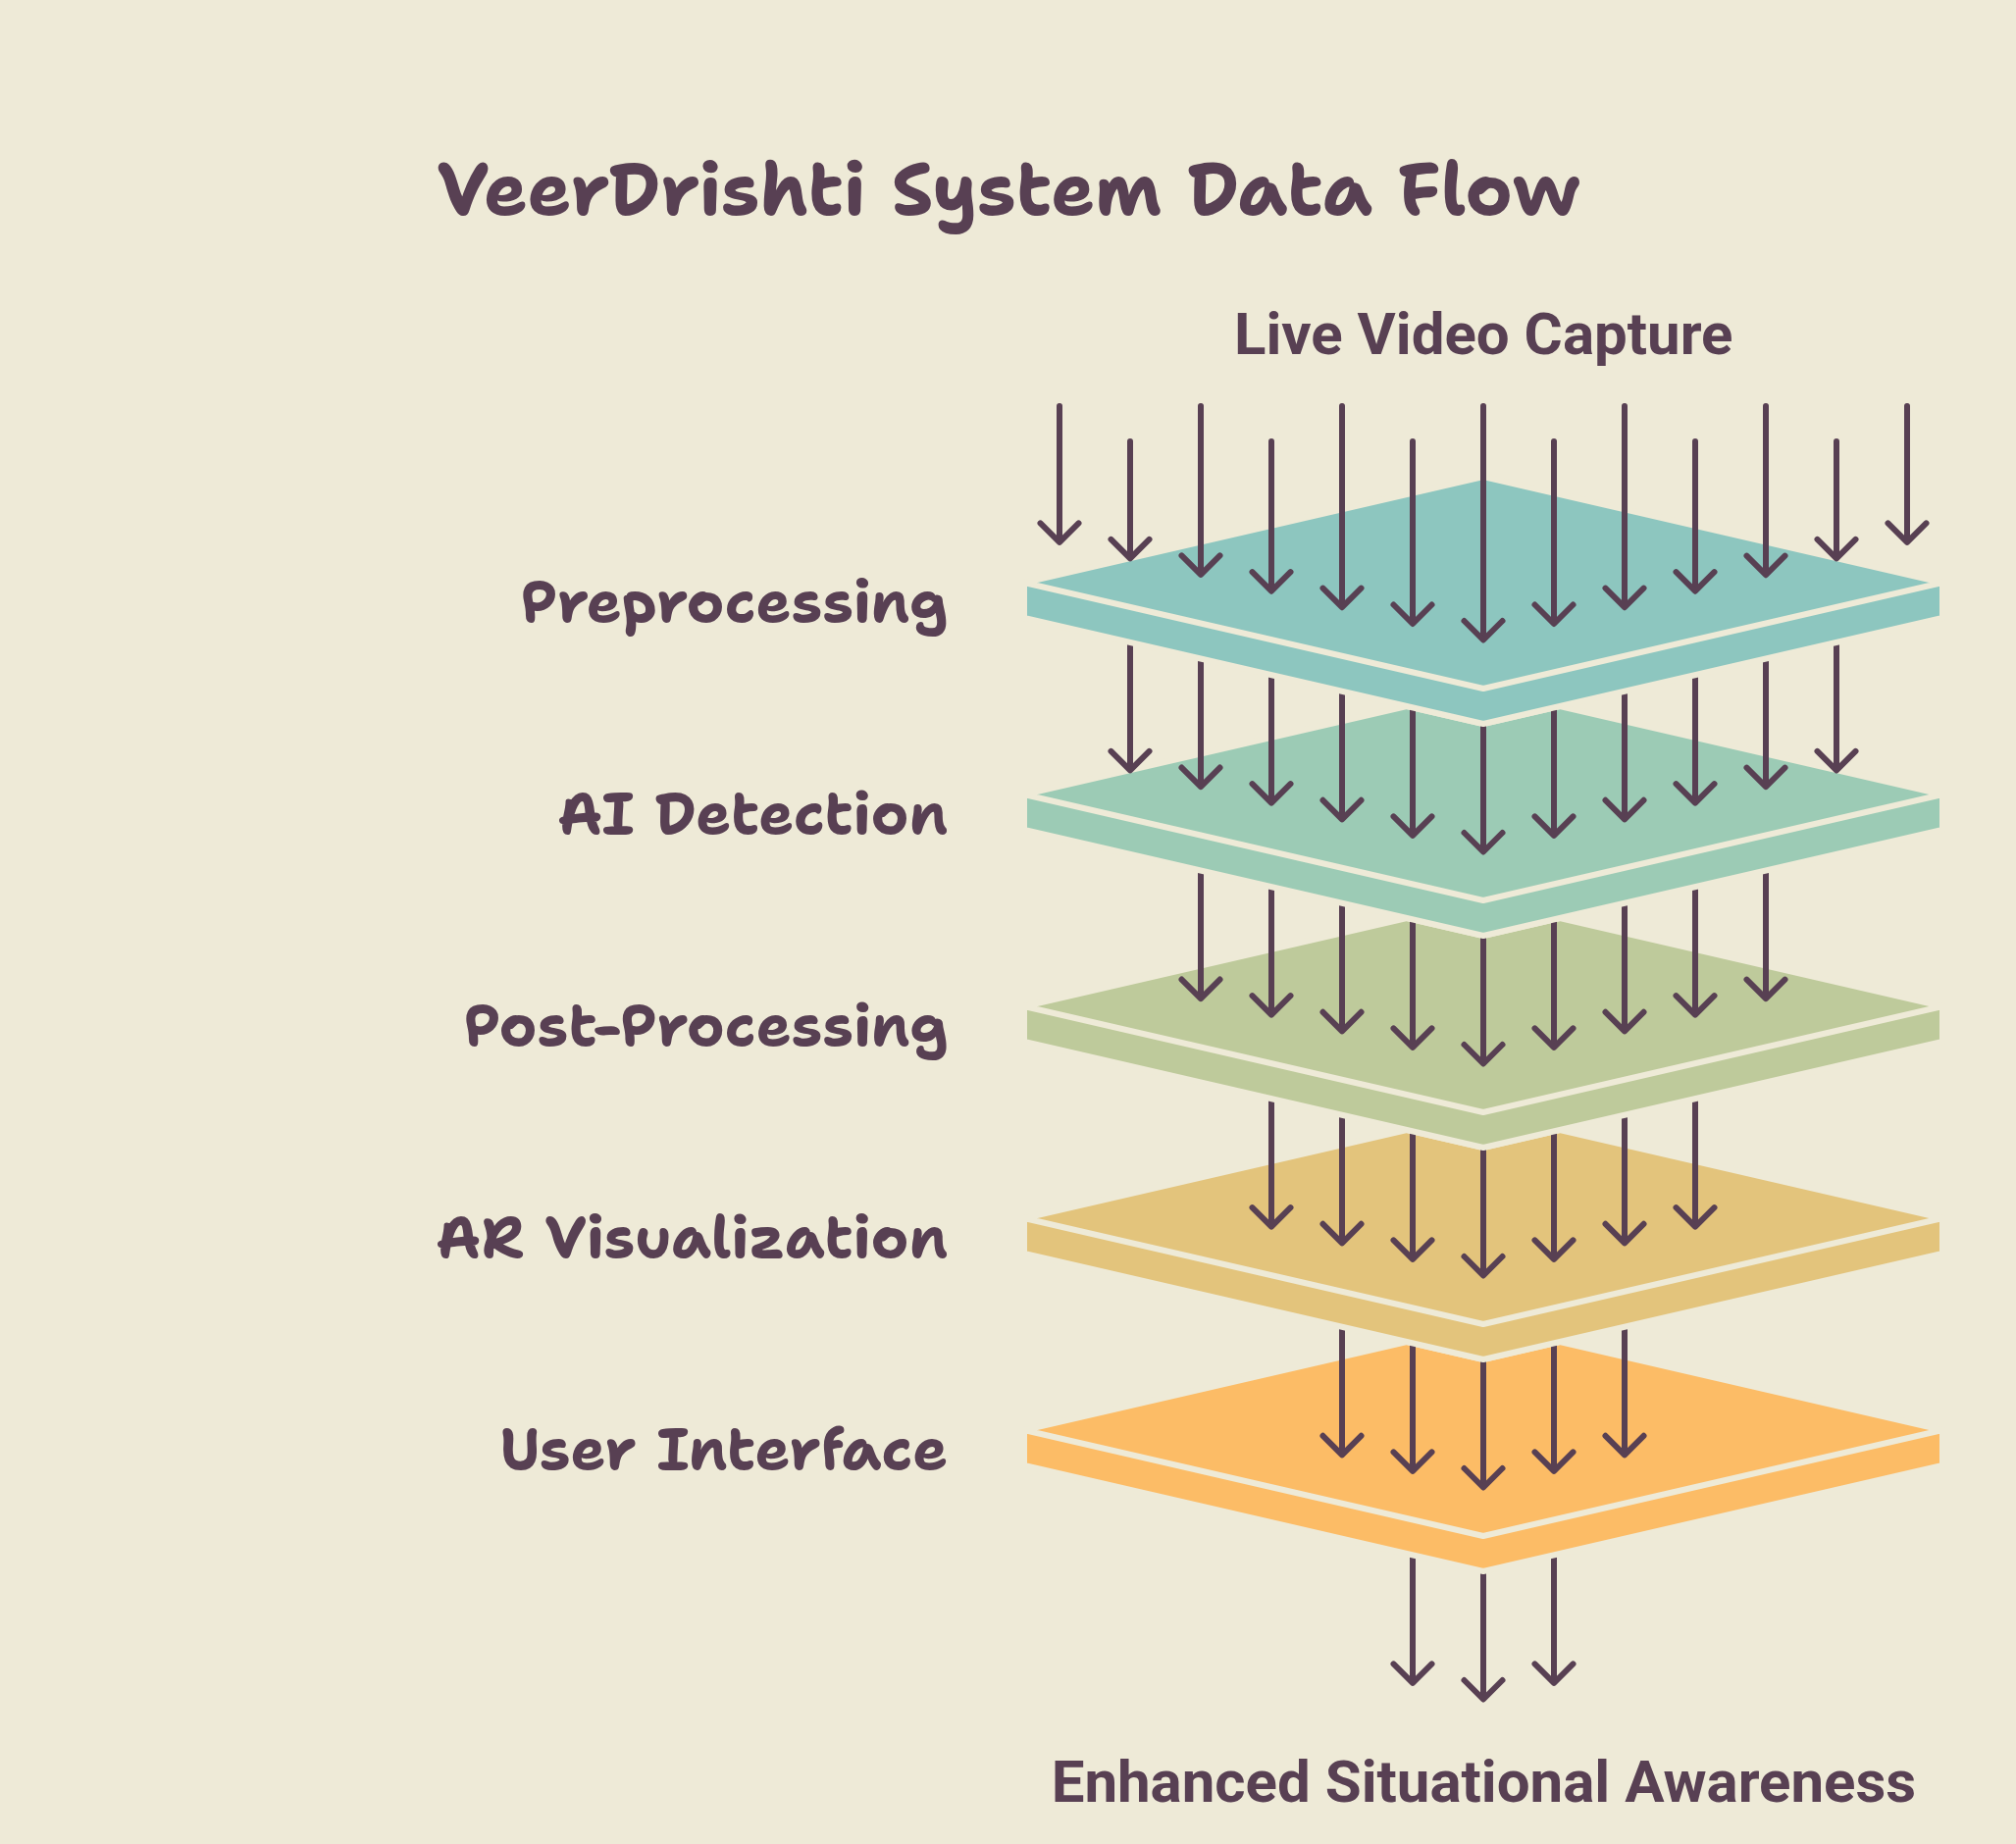
\includegraphics[width=0.62\textwidth]{images/architecture.png}
  \caption{System Architecture}\label{fig:architecture}
\end{figure}

In the prototype, CameraX supplies frames, the native YOLO pipeline prepares and analyzes them,
and Flutter YOLOView renders the outputs. The design uses the term AR visualization for the
overlays; the demonstrated outputs show image-space boxes, masks, and keypoints rather than a
world-registered augmented-reality system. Logcat supports development diagnostics independently
of the visual pipeline. Persistent mission storage is a proposed extension, not a demonstrated
layer of the current implementation.

\label{end:architecture}
\section{System Workflow}\label{sec:workflow}
Figure~\ref{fig:workflow} presents the operational workflow. The sequence
starts with RGB camera input and proceeds through preprocessing, model execution,
post-processing, user-interface visualization, and interpretation of the displayed output.

\begin{figure}[htbp]
  \centering
  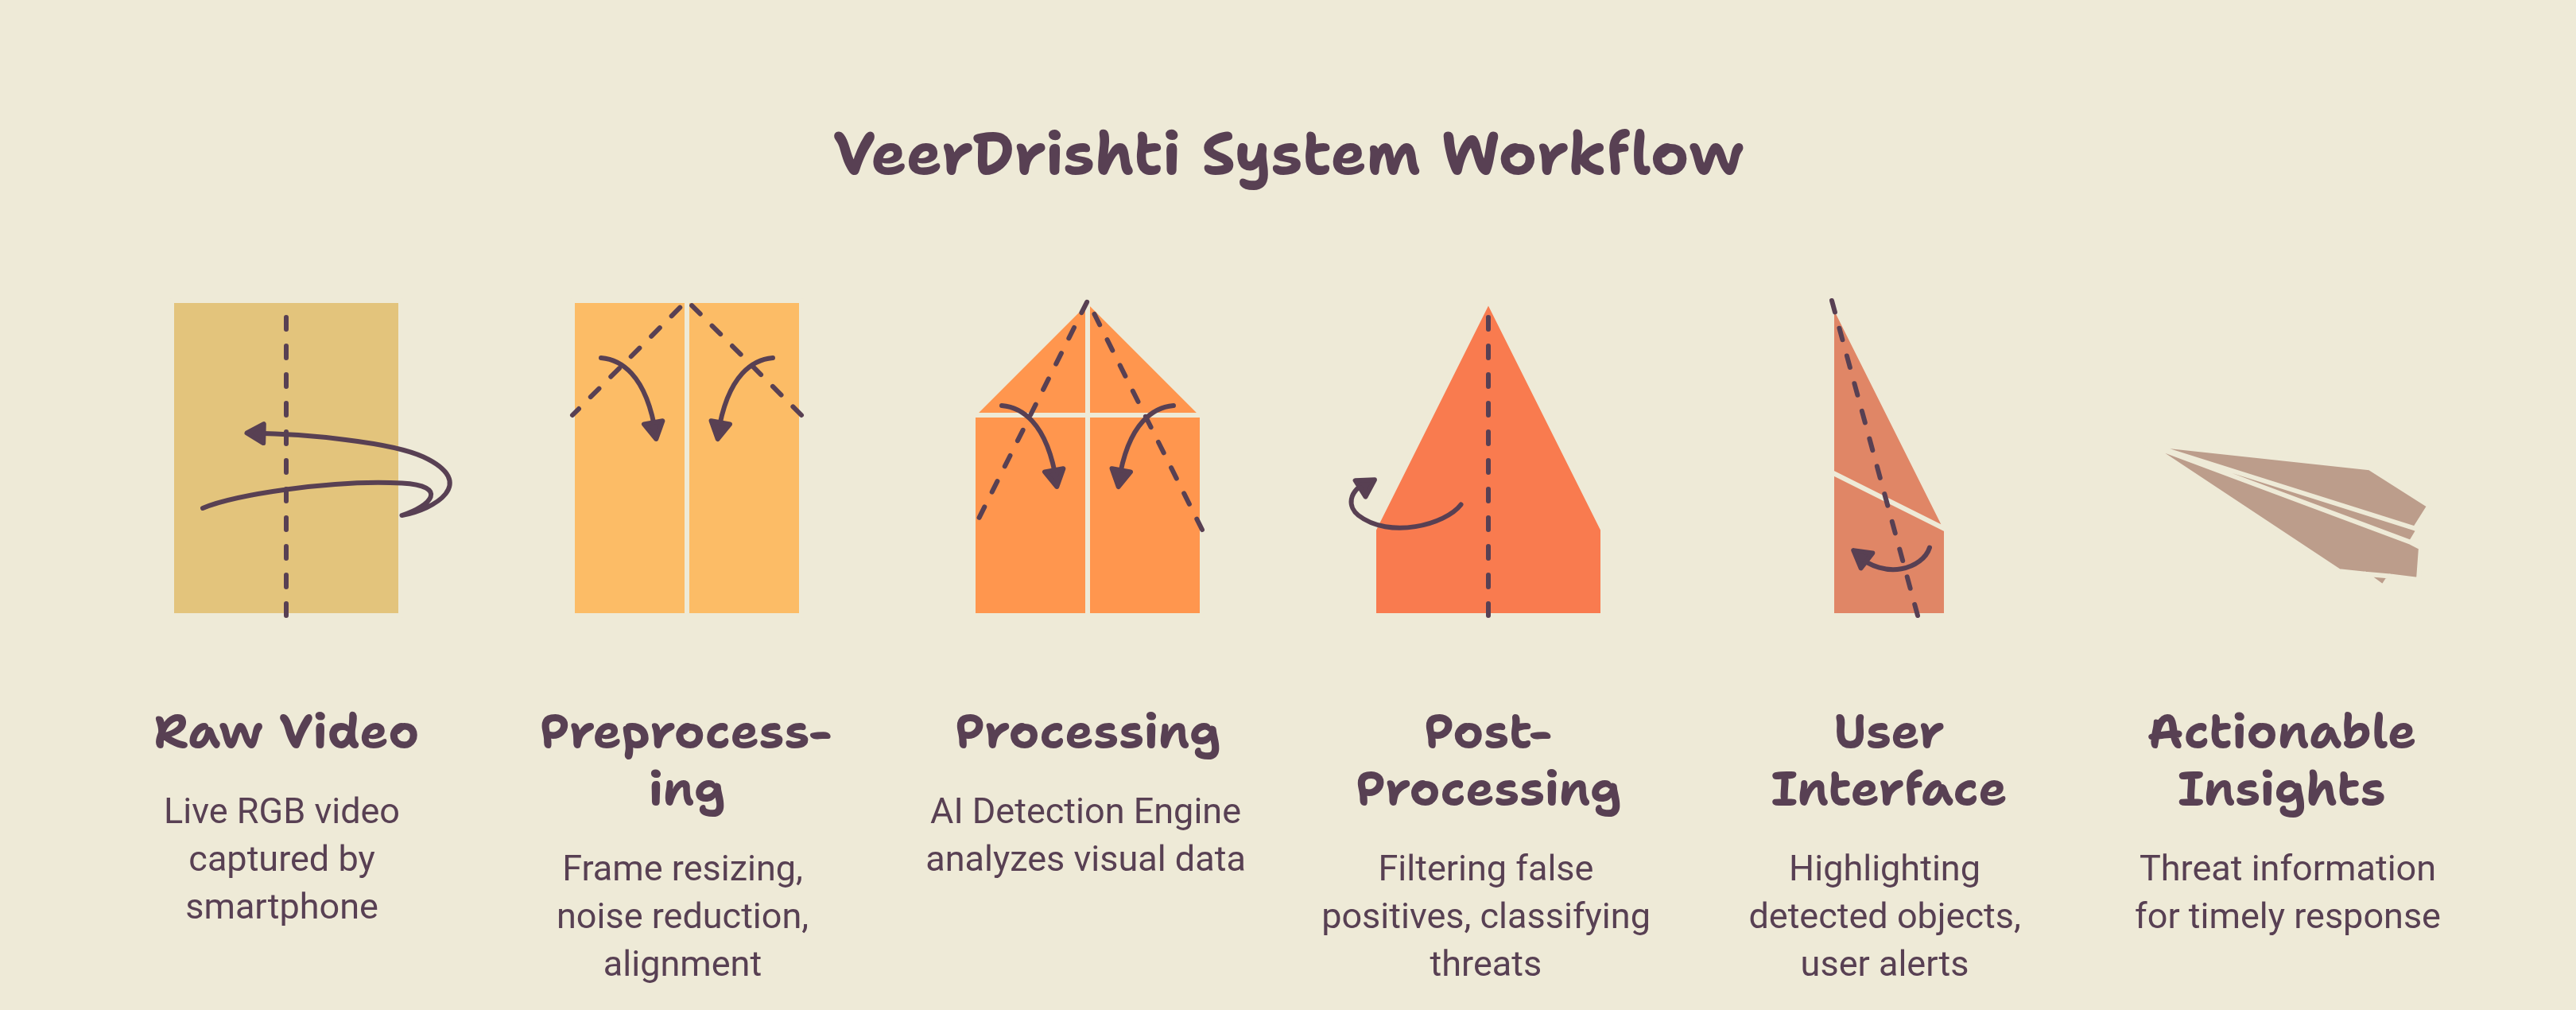
\includegraphics[width=\textwidth]{images/workflow.png}
  \caption{System Workflow}\label{fig:workflow}
\end{figure}

The implemented preprocessing operations are rotation, resizing or letterboxing, RGB conversion,
and tensor preparation. After inference, filtering settings and coordinate mapping determine
which outputs are drawn on the preview. The detection, segmentation, and pose modes provide
different visual representations within this loop. The diagram's references to threat
classification and user alerts express the wider design objective; the demonstrated outputs
establish object-class overlays and do not demonstrate hostile-intent classification or a
separate alerting service.
\label{end:workflow}\label{end:design}
\par\endgroup
